\documentclass[preview=true]{standalone}
\pdfinfoomitdate=1
\pdftrailerid{}
\pdfsuppressptexinfo=1
\usepackage{tikz}
\usepackage{pgfplots}
\usetikzlibrary{patterns}
\pgfplotsset{compat=1.16}
\begin{document}
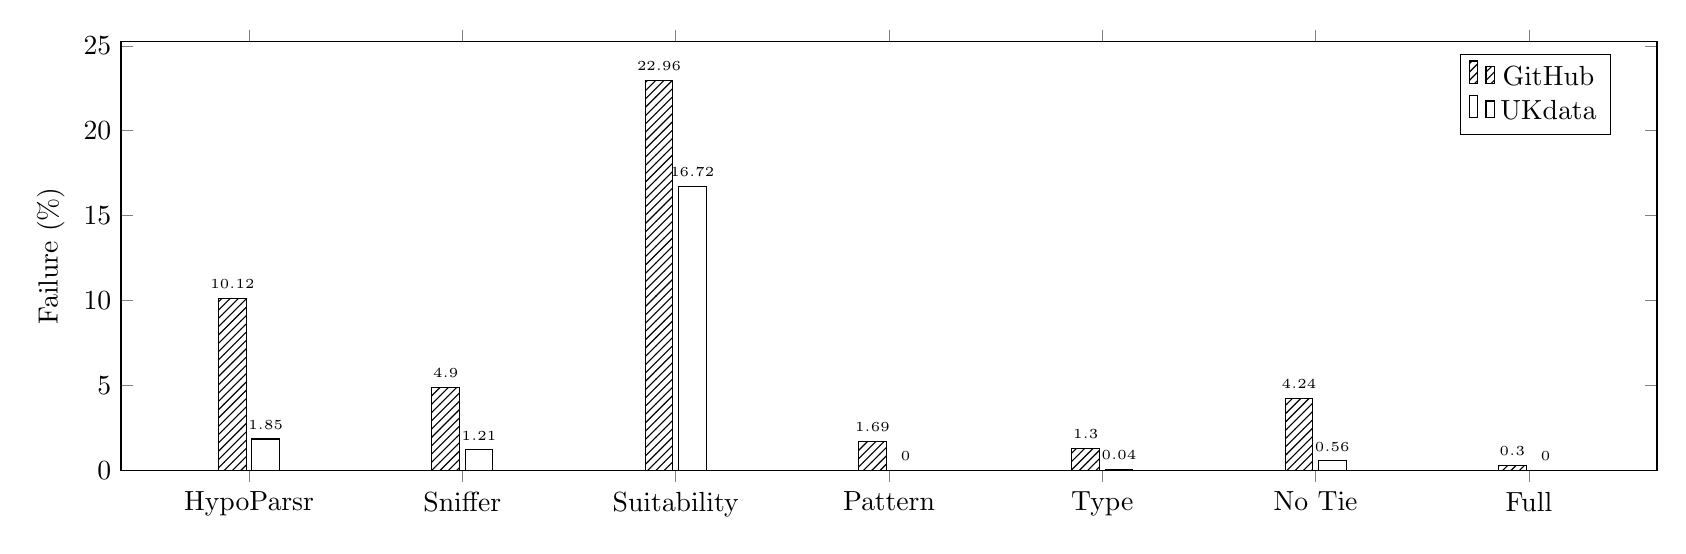
\begin{tikzpicture}
\begin{axis}[
	ybar,
	width={600},
	height={200},
	ymin=0,
	legend pos={north east},
	ylabel={Failure (\%)},
	symbolic x coords={HypoParsr,Sniffer,Suitability,Pattern,Type,No Tie,Full},
	xtick=data,
	nodes near coords,
	every node near coord/.append style={font=\tiny, /pgf/number format/fixed},
	nodes near coords align={vertical},
	]
\addplot[postaction={pattern=north east lines}] coordinates {(HypoParsr,10.1231190150478803) (Sniffer,4.9019607843137258) (Suitability,22.9594163246694016) (Pattern,1.6871865025079800) (Type,1.2995896032831737) (No Tie,4.2407660738714092) (Full,0.2963976288189695) };
\addplot[postaction={pattern=none}] coordinates {(HypoParsr,1.8514791708593277) (Sniffer,1.2074864157778227) (Suitability,16.7236868585228393) (Pattern,0.0000000000000000) (Type,0.0402495471925941) (No Tie,0.5634936606963171) (Full,0.0000000000000000) };
\legend{GitHub, UKdata}
\end{axis}
\end{tikzpicture}
\end{document}